\documentclass[12pt]{article}
\usepackage{fancyhdr}
\usepackage[margin=1in]{geometry}
\usepackage{indentfirst}
\usepackage{graphicx,wrapfig,afterpage}
\usepackage{hyperref}
\usepackage{adjustbox}
\usepackage{textgreek}
\usepackage{subcaption}
\usepackage{graphicx}
\usepackage{siunitx}

\pagestyle{fancy}
\fancyhf{}
\fancyhead[LE,RO]{Anmol Modur}
\fancyhead[RE,LO]{Robotic Systems: Lab 2}
\fancyfoot[CE,CO]{\leftmark}
\fancyfoot[LE,RO]{\thepage}

\usepackage{xcolor}
\usepackage{listings,lstautogobble}
\lstset
{
    language=C++,
    breaklines=true,
    basicstyle=\tt\scriptsize,
    keywordstyle=\color{blue},
    identifierstyle=\color{cyan},
    commentstyle=\color{gray},
    stringstyle=\ttfamily\color{green},
    autogobble=true,
    xleftmargin=0.5in,
    xrightmargin=0.5in,
}

\begin{document}
\begin{titlepage}
	\centering
	\vspace*{1.5in}
	{\Huge\bfseries Robotic Systems\par}
	\vspace{1in}
	{\scshape\LARGE\bfseries Lab 2\par}
	\vspace{2in}
	{\Large\itshape by Anmol Modur}
	\vfill

	{\large \today\par}
\end{titlepage}

\tableofcontents
\newpage
\section{Purpose}

The purpose of this lab is to get the student familiar with embedded systems and microcontrollers. This lab will cover analog and digital signals and how to interact with them using a microcontroler. By the end of this lab, the student will be able to recreate any of the examples in this lab as well as demonstrate their ability to perform tasks with the microcontroller. 

\section{Introduction}

Analog and Digital signals are the basis to any electronic system. They carry information, power instruments, control mechanical devices and more. Being able to understand these signals is complex, but being able to control these signals is even harder. With the introduction of processors and controllers, they make this task much easier. Sending instructions to the processor or controller to make the system perform exactly as specified is one feature people can't live without. No matter how complicated the signal is, there may be a controller for it. 

In this lab we aim to look at microcontrollers in particular. These microcontrollers are designed in general to deal with low power signals.

\subsection{Digital Signals}

Digital Signals are the essence of any digital based system. These signal operate by providing a discrete signal to communicate information. Digital signals are easy to work with as controllers and processors only use digital signals. These signals are used when information is needed to be stored, and have a greater signal to noise ratio. Communicating with digital signal is simple and almost any controller can do it. 

Digital signals often have ranges for acceptable high and low signal levels. Inputs often have more tolerance for acceptable levels. This is to account for signal degradation in high signals and noise in low signals. Figure \ref{fig:TTL} shows the Transistor Transistor Logic (TTL) levels for a \SI{5}{\volt} system. \textbf{Note: The Teensy 4.0 operates at \SI{3.3}{\volt}. Feeding anything higher into the controller may damage or fry your controller}.

\begin{figure}[h]
    \centering
    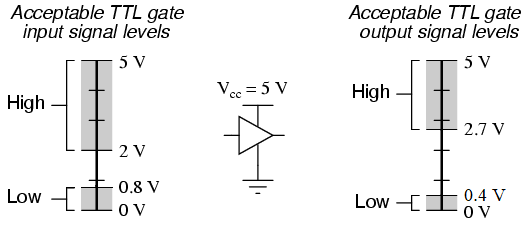
\includegraphics[width=0.5\textwidth]{TTL_Levels.png}
    \caption{TTL Levels}
    \label{fig:TTL}
\end{figure}

\subsubsection{Pull Up and Pull Down Networks}

When reading a digital input from a device such as a switch or button, the pin can be floating when there is no contact in the button or switch. This mean the voltage at that pin could either be read high or low by the microcontroller. To eliminate the uncertainty. A pull up or pull down network is used. When using an active high switch, the switch is connected to the source level, and a pull down resistor is connected to ground. When the switch is not active or pressed, the resistor pulls the output low. When the switch is active, the output gets pulled high since there is no resistance in the path to the source. The same principle applies to a pull up resistor, which is used with an active low switch.

\begin{figure}[h]
    \centering
    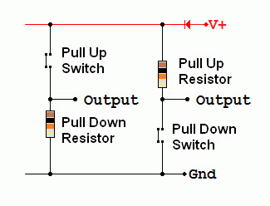
\includegraphics[width=0.5\textwidth]{pull_up_network.png}
    \caption{Pull-up and Pull-down Networks}
    \label{fig:pull up Pull down}
\end{figure}

\subsubsection{Interrupts}

There are two ways to read a digital input. The first way is to poll for an input. When polling, the microcontroller checks the values of the input signals, often by reading them. It then performs actions based on those values. The reading and handling of the signals is done in the main program.

The other method is by using interrupts. Interrupts are often ``attached'' to specified pins. When the state of that pin changes, the handler of the interrupts tells the main program to pause, and then run the interrupt state routine (ISR). The ISR is a function that immediately runs when interrupt is triggered. Unlike other functions, it cannot be called by the main program. The response to the input signal is then done in the ISR. after the ISR finishes, the main program resumes from when it was interrupted. Interrupts only work for digital pins.

Interrupts don't only have to be for external signals such as switches. They can also be triggered by other devices such as timers and analog to digital converters (ADCs). 

\begin{figure}
     \centering
     \begin{subfigure}{0.45\textwidth}
         \centering
         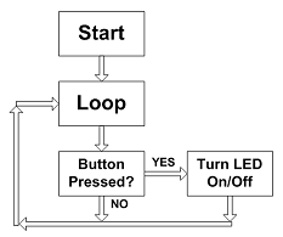
\includegraphics[width=\textwidth]{polling.png}
         \caption{Polling}
         \label{fig:polling}
     \end{subfigure}
     \hfill
     \begin{subfigure}{0.45\textwidth}
         \centering
         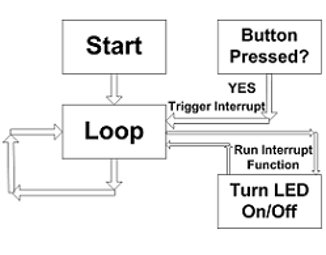
\includegraphics[width=\textwidth]{interrupts.png}
         \caption{Interrupts}
         \label{fig:interrupts}
     \end{subfigure}
     \caption{Flowcharts for Polling and Interrupts}
     \label{fig:polling and interrupts}
\end{figure}


\subsubsection{Button Bouncing}

When pressing physical buttons, the transition of the signal from high to low is not perfect. It often bounces from high to low for a brief period before it settles. This can sometimes lead to controllers incorrectly detecting button presses. The way of handling this so that multiple presses aren't detected is called denouncing. 

\begin{figure}[h]
    \centering
    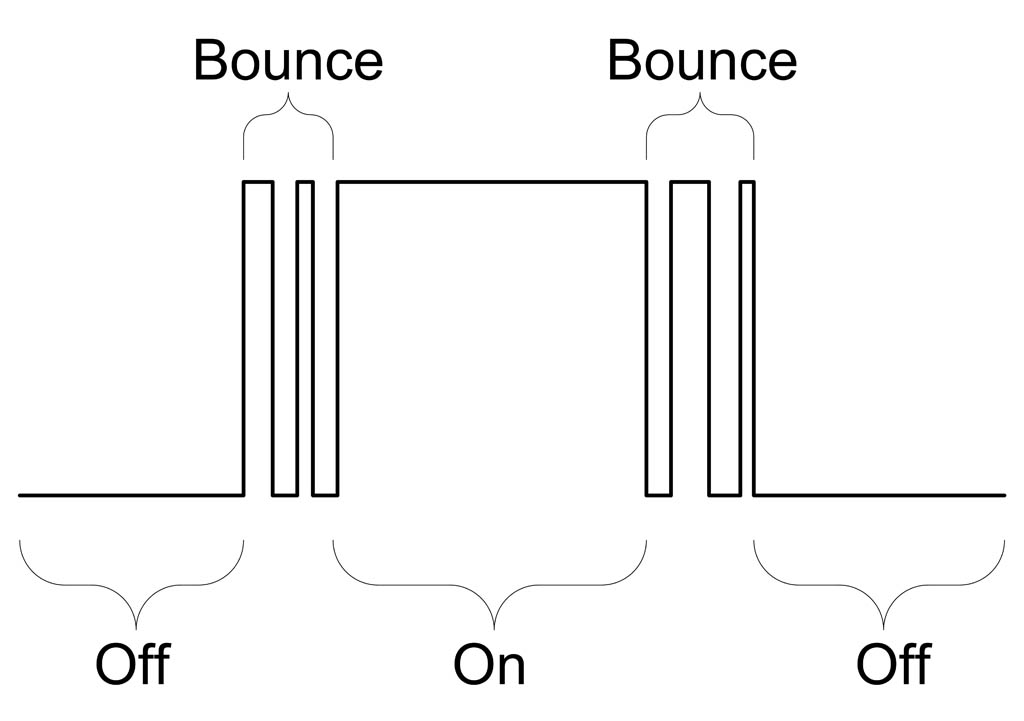
\includegraphics[width=0.5\textwidth]{bouncing.jpg}
    \caption{Button Bouncing}
    \label{fig:bouncing}
\end{figure}


\subsection{Analog Signals}

Analog signal are the natural signals of the world. These signals are often continuous compared to the discrete nature of digital signals. Information through analog signals is usually more complicated than in digital signals as the information is embedded in the signal's properties.

\begin{figure}[h]
    \centering
    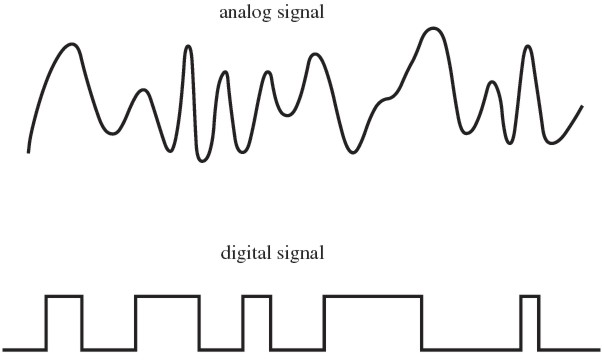
\includegraphics[width=0.5\textwidth]{signals.jpg}
    \caption{Analog and Digital Signals}
    \label{fig:bouncing}
\end{figure}

\subsubsection{ADCs and DACs}


An ADC is an analog to digital converter. It allows micorocontrollers to read analog signals. It takes in a reading, or sample of a signal, and then quantizes it to a finite set of levels, essentially converting it to a discrete signal. The amount of levels is determined by the bit-resolution of the ADC. An $n$-bit ADC has $2^n$ levels that it can be quantized to. The precision of voltages that can be read depends on the resolution and the full scale voltage of the ADC. The ADC often has a range of voltages that it can read. For example, the Teensy 4.0 has an ADC range from \SI{0}{\volt} to \SI{3.3}{\volt}. Voltages outside this range may damage the ADC and possibly the microcontroller.  ADC's are essential for any processor or controller to communicate to the analog world. Without this, these processors and controllers would be next to useless.

\begin{figure}[h]
    \centering
    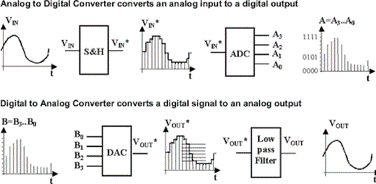
\includegraphics{adc_dac.png}
    \caption{ADC and DAC Operations}
    \label{fig:my_label}
\end{figure}

A DAC is a digital to analog converter. A DAC allows a controller to produce an exact analog voltage. It is similar to an ADC in that it has a bit resolution that determines the precision about what voltages it can create. While ADCs can be found on almost any microcontroller, DACs are not present on most microcontrollers, including the Teensy 4.0, due to them being more expensive. 


\subsubsection{Pulse Width Modulation}

Pulse Width Modulation (PWM) is another and more practical way for a microcontroller to produce an analog signal. This signal is simulated with a purely digital signal. A PWM signal is a pulse train with a on-time that can be modified. The ratio of on-time to the period of the signal is known as the duty cycle. By changing the duty cycle, the effective or average voltage of the signal changes. This allows the microcontroller to produce varying or analog voltages. This is very useful for changining the brightness of LEDs and adjusting the speeds of motors.

\begin{figure}[h]
    \centering
    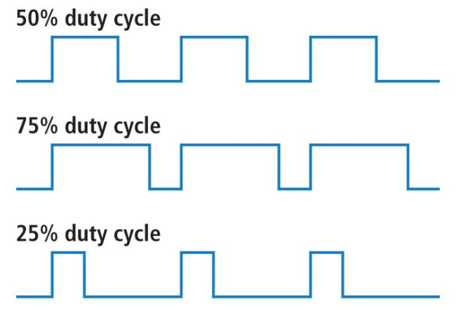
\includegraphics[width=0.7\textwidth]{PWM.png}
    \caption{PWM}
    \label{fig:PWM}
\end{figure}

For servos, PWM works a bit differently. There is a fixed period and the the position of the servo motor is dependent on the on-time of the pulse, instead of the duty cycle. For standard hobby servos, a typical range for on-times is usually between 1 and \SI{2}{\milli\second}, with \SI{1.5}{\milli\second} being for the mid point of the servo. These timings are also used for components that use R/C signals.

\begin{figure}[h]
    \centering
    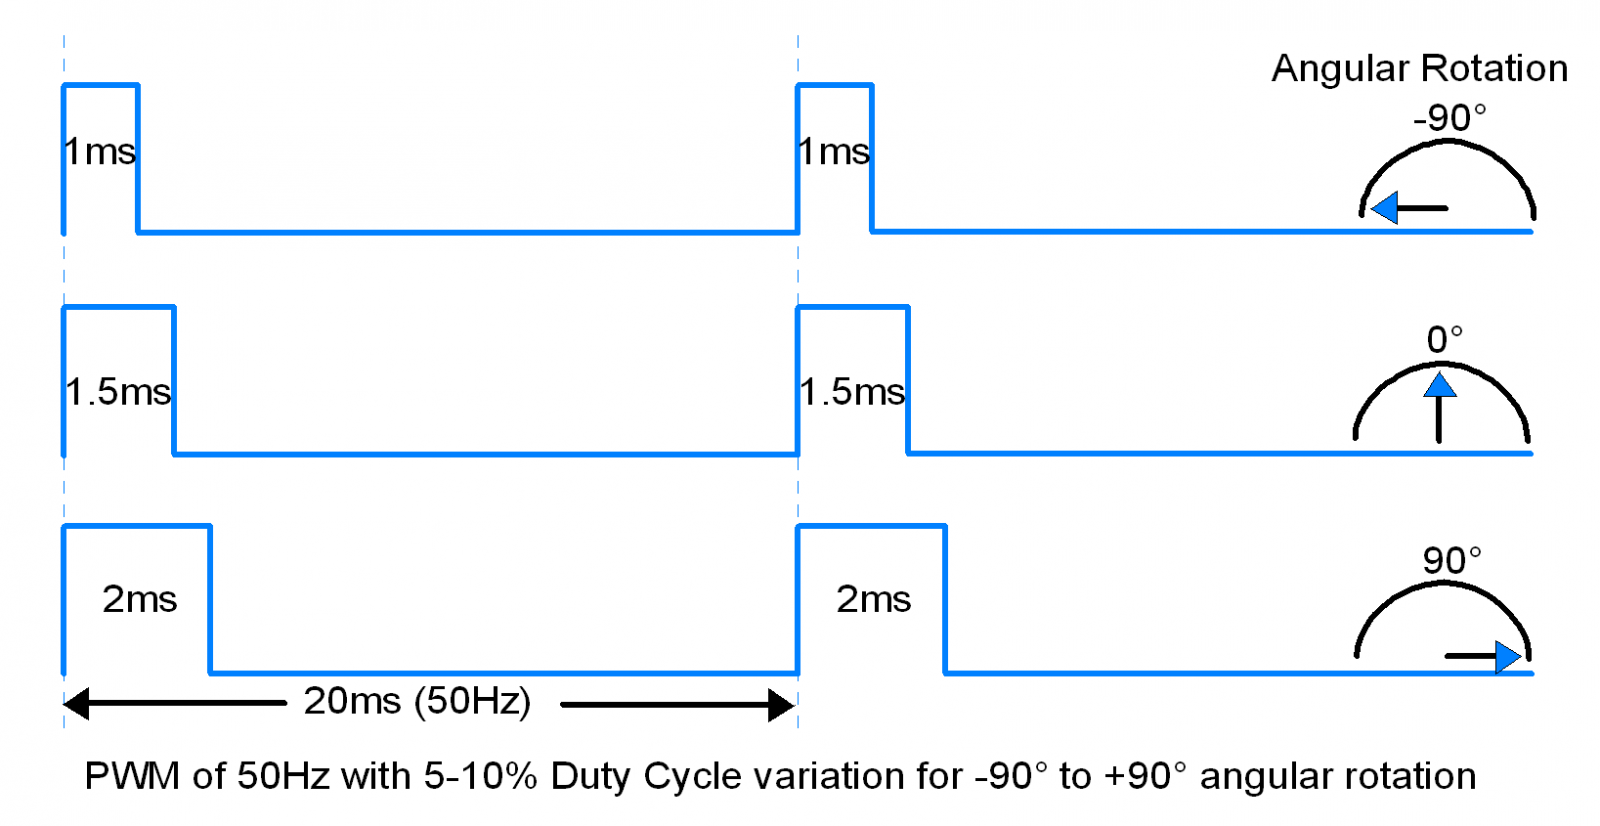
\includegraphics[width=0.7\textwidth]{Servo_PWM_Duty_Cycle.png}
    \caption{PWM for Servo Motors}
    \label{fig:Servo_PWM}
\end{figure}

\clearpage
\section{Lab Assignments}

Start this lab by downloading the zipped folder on mycourses. This should contain 6 Folders. Ensure Platform IO is installed correctly. Use the installation guide if necessary. To complete this lab, open each folder in order and complete the tasks asked. Show the TA the final result to get your check off. 

\bigskip
\textbf{Follow this order:}
\begin{enumerate}
\item Code - DO

Make the on-board LED blink at a rate of \SI{100}{\hertz}.

\item Potentiometer - AI

Modify the given code so that the values on the serial monitor a printing a percentage of how much the potentiometer has turned.

\item Dimming LED - AO

Modify the given code to generate a \SI{2}{\hertz} triangle signal and output it to the LED pin.

\item Interrupts - DI

Modify the given code so that the LED goes through a sequence of blinking at 1Hz, 2Hz, 3Hz, 4Hz and 5Hz every time the push button is pressed. The LED should begin blinking at \SI{1}{\hertz} and continue blinking at that rate until the microcontroller detects a button press. The same process would continue at \SI{2}{\hertz}. The rate should loop back to \SI{1}{\hertz} when a button press is detected at \SI{5}{\hertz}. Follow the flowchart in \ref{fig:interrupts_flowchart} for guidance. 

\begin{figure}
    \centering
    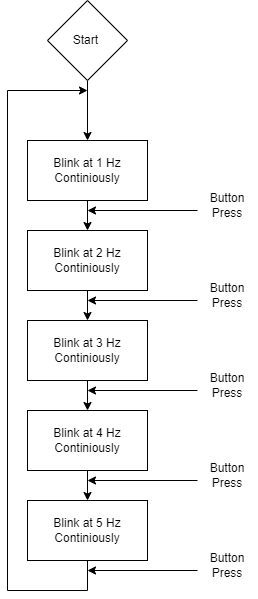
\includegraphics{Interrupts - DI.png}
    \caption{Interrupts - DI Flowchart}
    \label{fig:interrupts_flowchart}
\end{figure}

\item Servo

Modify the code to make servo oscillate from 0 - 2pi/3 radians every 5 seconds. The servo should be continuously moving throughout this period. 

\end{enumerate}

\clearpage
\section{Questions}

\begin{enumerate}
\item Give examples where interrupts should and shouldn't be used in a code.
\item Explain how a microcontroller can reproduce analog signals.
\item Why is C++ a preferred way to program microcontrollers instead of other languages?
\end{enumerate}

\section{Appendex}

Make sure to include and additional information in your report as specified in the lab documents.

\end{document}